\documentclass[a4paper]{article}

\usepackage{amsmath}
\usepackage{amssymb,amsfonts}
\usepackage[catalan]{babel} % Language 
\usepackage{fontspec}
\usepackage[margin=2cm]{geometry}
\usepackage{graphicx}
\usepackage[makeroom]{cancel}
\usepackage{listings}
\usepackage[dvipsnames]{xcolor}
\usepackage{float}
\usepackage[hidelinks]{hyperref}

\setlength{\parindent}{0pt}
\setlength{\parskip}{0.2cm}

\lstset{ % Donat que el paquest listings no té la sintaxi per R definida la hem de definir nosaltres
    language=R,                     % the language of the code
    basicstyle=\ttfamily\footnotesize,       % the size of the fonts that are used for the code
    numbers=left,                   % where to put the line-numbers
    numberstyle=\tiny\color{gray},  % the style that is used for the line-numbers
    stepnumber=1,                   % the step between two line-numbers. If it's 1, each line
    % will be numbered
    numbersep=5pt,                  % how far the line-numbers are from the code
    backgroundcolor=\color{white},  % choose the background color. You must add \usepackage{color}
    showspaces=false,               % show spaces adding particular underscores
    showstringspaces=false,         % underline spaces within strings
    showtabs=false,                 % show tabs within strings adding particular underscores
    frame=single,                   % adds a frame around the code
    rulecolor=\color{black},        % if not set, the frame-color may be changed on line-breaks within not-black text (e.g. commens (green here))
    tabsize=2,                      % sets default tabsize to 2 spaces
    captionpos=b,                   % sets the caption-position to bottom
    breaklines=true,                % sets automatic line breaking
    breakatwhitespace=false,        % sets if automatic breaks should only happen at whitespace
    title=\lstname,                 % show the filename of files included with \lstinputlisting;
    % also try caption instead of title
    keywordstyle=\color{blue},      % keyword style
    commentstyle=\color{OliveGreen},   % comment style
    stringstyle=\color{purple},      % string literal style
    escapeinside={\%*}{*)},         % if you want to add a comment within your code
    morekeywords={*,...}            % if you want to add more keywords to the set
} 

\title{\textsc{APA Problemes} \\ Problema 8 Mínims quadrats}
\author{Joan Marcè i Igual}
\date{}

\begin{document}
\maketitle

\textbf{Tenim una seqüència de números reals $x_1,...x_N$. Definim la funció:}

$$ f(x) = \frac{1}{N}\sum_{n=1}^N(x - x_n)^2 $$

\begin{enumerate}

\item \textbf{Demostreu que $f$ té un únic mínim a $x^* = \frac{1}{N} \sum_{n=1}^N x_n$ i interpreteu el resultat.}

Primer buscarem els extrems de la funció, per fer-ho buscarem $f'(x)$ i després comprovarem que aquests extrems són mínims i que correspon amb el valor dona't per l'enunciat.

$$ f'(x) = \frac{2}{N}\sum_{n=1}^N (x - x_n) = \frac{2}{N}\left(\sum_{n=1}^N x - \sum_{n=1}^N x_n \right) = \frac{2}{N}\left(Nx - \sum_{n=1}^N x_n \right) = \underline{\underline{2x - \frac{2}{N}\sum_{n=1}^N x_n}} $$

$$ f'(x^*) = 0 \implies 2x^* - \frac{2}{N}\sum_{n=1}^N x_n = 0 \implies \boxed{x^* = \frac{1}{N}\sum_{n=1}^N x_n} $$

Així trobem un extrem de $f(x)$ ara hem de demostrar que és un mínim. Per tant, buscarem $f''(x)$ i comprovarem que $f''(x^*) > 0$.

$$ f''(x) = 2 \implies f''(x^*) > 0 $$

Així doncs queda demostrat que $x^*$ és un mínim (mentre $ N \ne \infty $).

\item \textbf{Considereu ara la nova funció:}

$$ f(x) = \sum_{n=1}^N p_n (x - x_n)^2 $$

\textbf{on ponderem cada $x_n$ per un factor $p_n > 0$ que compleix $\sum_{n=1}^N p_n = 1$. Recalculeu la solució. Comproveu que es redueix al cas anterior quan $p_n = 1/N$.}

Aplicarem el mateix mètode que a l'apartat anterior. Primer buscarem $f'(x)$ i obtindrem els extrems i, a continuació, comprovarem que aquests extrems siguin mínims a partir de $f''(x)$

$$ 
f'(x) = \frac{2}{N} \sum_{n=1}^N p_n(x - x_n) = 
\frac{2}{N}\left(\sum_{n=1}^N p_n x - \sum_{n=1}^N p_n x_n\right) = 
\frac{2}{N}\left(x\sum_{n=1}^N p_n - \sum_{n=1}^N p_n x_n\right) = 
\underline{\underline{\frac{2}{N}\left(x - \sum_{n=1}^N p_n x_n\right)}} 
$$
$$
f'(x) = 0 \implies \cancel{\frac{2}{N}}\left(x^* - \sum_{n=1}^N p_n x_n\right) \implies
\boxed{x^* = \sum_{n=1}^N p_n x_n}
$$
$$
\text{Si } p_n = \frac{1}{N} \implies \boxed{x^* = \frac{1}{N}\sum_{n=1}^N x_n}
$$

Ara que hem trobat un extrem de $f(x)$ buscarem $f''(x)$ per comprovar que és un mínim veient que $f''(x^*) > 0$.

$$
f''(x) = \frac{2}{N}\sum_{n=1}^N p_n = \frac{2}{N} \implies f''(x^*) > 0
$$

\item \textbf{[R] Apliqueu el darrer resultat a una seqüència de 1.000 nombres independents Gaussians de mitjana zero i desviació tipus 2. Useu una ponderació basada en nombres independents uniformes en (0,1).}

Si desenvolupem una mica la funció podrem veure que ens queda un polinomi de 2n grau:

$$
f(x) = \frac{1}{N} \sum_{n=1}^N (x - x_n)^2 =
\frac{1}{N} \sum_{n=1}^N p_n \left( x^2 - 2x_n x + x_n^2 \right) =
\frac{1}{N} \left( \sum_{n=1}^N p_n x^2 - 2\sum_{n=1}^N p_n x_n x + \sum_{n=1}^N p_n x_n^2 \right)=
$$
$$
\underbrace{\frac{1}{N}}_a x^2 - x \underbrace{\frac{2}{N}\sum_{n=1}^N p_n x_n}_b + \underbrace{\frac{1}{N}\sum_{n=1}^N p_n x_n^2}_c
$$

A la \autoref{fig:grafic} es pot veure la funció trobada i com hi ha un mínim proper al 0.

\vspace{0.5cm}

\lstinputlisting[language=R]{problema_1.R}

\begin{figure}[H]
    \centering
    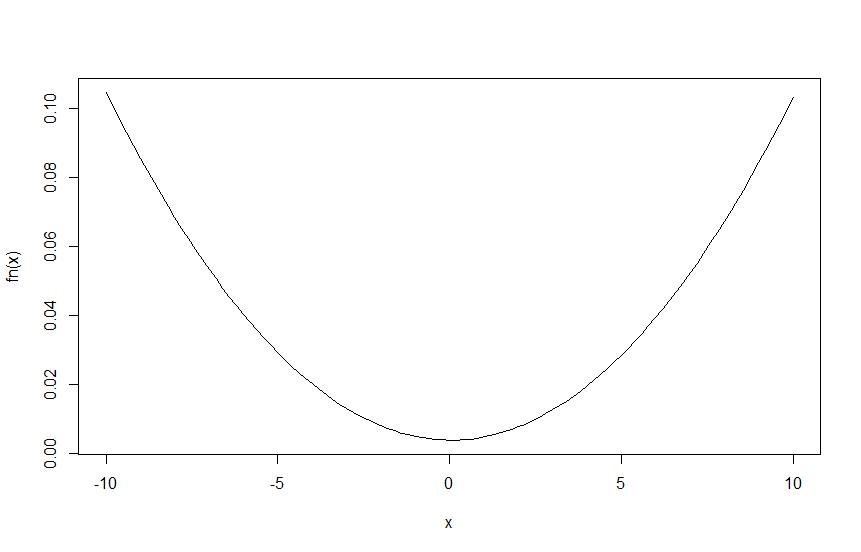
\includegraphics[width=0.5\linewidth]{problema_1_plot}
    \caption{Gràfic de la funció generat per R}
    \label{fig:grafic}
\end{figure}

\end{enumerate}

\end{document}